% This is the Duke University Statistical Science LaTeX thesis template.
% It has been adapted from the Reed College LaTeX thesis template. The
% adaptation was done by Mine Cetinkaya-Rundel (MCR). Some of the comments
% that are specific to Reed College have been removed.
%
% Most of the work on the original Reed College document class and template
% was done by Sam Noble (SN). Later comments etc. by Ben Salzberg (BTS).
% Additional restructuring and APA support by Jess Youngberg (JY).
%
% See https://www.reed.edu/cis/help/latex/ for help. There are a
% great bunch of help pages there, with notes on
% getting started, bibtex, etc. Go there and read it if you're not
% already familiar with LaTeX.
%
% Any line that starts with a percent symbol is a comment.
% They won't show up in the document, and are useful for notes
% to yourself and explaining commands.
% Commenting also removes a line from the document;
% very handy for troubleshooting problems. -BTS

%%
%% Preamble
%%
% \documentclass{<something>} must begin each LaTeX document
\documentclass[12pt,twoside]{dukestatscithesis}
% Packages are extensions to the basic LaTeX functions. Whatever you
% want to typeset, there is probably a package out there for it.
% Chemistry (chemtex), screenplays, you name it.
% Check out CTAN to see: http://www.ctan.org/
%%
\usepackage{graphicx,latexsym}
\usepackage{amsmath}
\usepackage{amssymb,amsthm}
\usepackage{longtable,booktabs,setspace}
\usepackage{chemarr} %% Useful for one reaction arrow, useless if you're not a chem major
\usepackage[hyphens]{url}
% Added by CII
\usepackage{hyperref}
\usepackage{lmodern}
\usepackage{float}
\floatplacement{figure}{H}
% End of CII addition
\usepackage{rotating}

% Next line commented out by CII
%%% \usepackage{natbib}
% Comment out the natbib line above and uncomment the following two lines to use the new
% biblatex-chicago style, for Chicago A. Also make some changes at the end where the
% bibliography is included.
%\usepackage{biblatex-chicago}
%\bibliography{thesis}


% Added by CII (Thanks, Hadley!)
% Use ref for internal links
\renewcommand{\hyperref}[2][???]{\autoref{#1}}
\def\chapterautorefname{Chapter}
\def\sectionautorefname{Section}
\def\subsectionautorefname{Subsection}
% End of CII addition

% Added by CII
\usepackage{caption}
\captionsetup{width=5in}
% End of CII addition

% \usepackage{times} % other fonts are available like times, bookman, charter, palatino


% To pass between YAML and LaTeX the dollar signs are added by CII
\title{}
\author{}
% The month and year that you submit your FINAL draft TO THE LIBRARY (May or December)
\date{}
\advisor{}
\institution{}
\degree{}
\committeememberone{}
\committeemembertwo{}
\dus{}
%If you have two advisors for some reason, you can use the following
% Uncommented out by CII
% End of CII addition

%%% Remember to use the correct department!
\department{}

% Added by CII
%%% Copied from knitr
%% maxwidth is the original width if it's less than linewidth
%% otherwise use linewidth (to make sure the graphics do not exceed the margin)
\makeatletter
\def\maxwidth{ %
  \ifdim\Gin@nat@width>\linewidth
    \linewidth
  \else
    \Gin@nat@width
  \fi
}
\makeatother

\renewcommand{\contentsname}{Table of Contents}
% End of CII addition

\setlength{\parskip}{0pt}

% Added by CII

\providecommand{\tightlist}{%
  \setlength{\itemsep}{0pt}\setlength{\parskip}{0pt}}

\Acknowledgements{

}

\Dedication{

}

\Preface{

}

\Abstract{

}

% End of CII addition
%%
%% End Preamble
%%
%

\usepackage{amsthm}
\newtheorem{theorem}{Theorem}[chapter]
\newtheorem{lemma}{Lemma}[chapter]
\theoremstyle{definition}
\newtheorem{definition}{Definition}[chapter]
\newtheorem{corollary}{Corollary}[chapter]
\newtheorem{proposition}{Proposition}[chapter]
\theoremstyle{definition}
\newtheorem{example}{Example}[chapter]
\theoremstyle{definition}
\newtheorem{exercise}{Exercise}[chapter]
\theoremstyle{remark}
\newtheorem*{remark}{Remark}
\newtheorem*{solution}{Solution}
\begin{document}

% Everything below added by CII

\frontmatter % this stuff will be roman-numbered
\pagestyle{empty} % this removes page numbers from the frontmatter



  \hypersetup{linkcolor=black}
  \setcounter{tocdepth}{2}
  \tableofcontents





\mainmatter % here the regular arabic numbering starts
\pagestyle{fancyplain} % turns page numbering back on

\chapter{Data}\label{data}

\section{Description of Dataset}\label{description-of-dataset}

The data for this analysis comes from SportVU, a player-tracking system
from STATS, LLC. that provides precise coordinates for all ten players
and the ball at a rate of 25 times per second. The Duke University Men's
Basketball team permitted us to use their SportVU data from the 2014 to
2017 basketball seasons for this project. Since the ability to record
this data depends on specialized tracking cameras, Duke does not have
this data for every game they play---only home games, and a few road
games in arenas that had the techology installed. Therefore, there is a
substantial amount of missing data between games. More specifically,
between the 2014 and 2017 seasons, the Duke Men's Basketball team played
147 games; this dataset contains 94 games, with 82 at Duke and 12 on
another court.

For our analysis, we use the following files for each game:
\begin{itemize}
\tightlist
\item
  Final Sequence Play-by-Play Optical:
\end{itemize}
This dataset comes in an a semi-structured Extensible Markup Language
(XML) file, where there is a unique element for each ``event'' (an event
is a basketball action such as a dribble, pass, shot, foul, etc.). Each
event element has attributes describing the type of event, the time of
the event, and the player who completed the action. We use these files
to uncover when a shot is attempted in a game, who attempted the shot,
and the result of the shot attempt.
\begin{itemize}
\tightlist
\item
  Box Score Optical:
\end{itemize}
We use this dataset to match the names and IDs of players who are in the
game. This is also an XML file, with elements corresponding to
individual players. These elements contain attributes describing
information about the player (e.g.~team name, jersey number) and various
statistics for the game (e.g.~points, assists, distance run).
\begin{itemize}
\item
  Final Sequence Optical:

  These XML files contain the locations of all ten players and the ball
  during precise time intervals within the game. Each timeunit has a
  unique element, and these elements have attributes describing the
  locations. We merge this with the Final Sequence Play-by-Play Optical
  data on the time attribute to obtain the shooter's location at the
  moment of a shot attempt.
\end{itemize}
\section{Data Cleaning}\label{data-cleaning}

Steps taken to clean the merged shooter IDs with shot locations include
standardizing the locations onto a half-court setting (the teams switch
sides of the court halfway through every game, which means that we have
to flip the coordinates across the middle of the court for half of the
data in every game), converting the x-y coordinates to polar coordinates
(in the units of feet and radians), and including an indicator for home
games. The final dataset had 5467 observations from 31 shooters over 94
games. A summary of the cleaned dataset is in Table
\ref{tab:tablesummary}:
\begin{longtable}[]{@{}llll@{}}
\caption{\label{tab:tablesummary}Summary of Dataset}\tabularnewline
\toprule
Name & Type & Values & Extra Details\tabularnewline
\midrule
\endfirsthead
\toprule
Name & Type & Values & Extra Details\tabularnewline
\midrule
\endhead
season & categorical & \{2014, \ldots{}, 2017\} &\tabularnewline
gameid & categorical & NA & 94 unique values\tabularnewline
time & continuous & NA & 13-digit timestamp in
milliseconds\tabularnewline
globalplayerid & categorical & NA & 31 unique values\tabularnewline
r & continuous & {[}0, \(\infty\)) & Distance of shot from hoop
(feet)\tabularnewline
theta & continuous & {[}-\(\pi\), \(\pi\){]} & Angle of shot
(radians)\tabularnewline
home & categorical & \{0,1\} & 1 if shot occured during a home
game\tabularnewline
result & categorical & \{0,1\} & 1 if shot was
made(response)\tabularnewline
\bottomrule
\end{longtable}
and a small subset of the cleaned data is displayed below in Table
\ref{tab:tablesample}:

\begingroup\fontsize{11}{13}\selectfont
\begin{longtable}[t]{rllrrrrr}
\caption[Data Sample]{\label{tab:tablesample}Sample of Dataset}\\
\toprule
season & gameid & time & globalplayerid & r & theta & home & result\\
\midrule
2014 & 201401070173 & 1389141733839 & 603106 & 4.2076 & 1.0746 & 1 & 1\\
2014 & 201401070173 & 1389141844712 & 601140 & 16.6537 & 1.2973 & 1 & 0\\
2014 & 201401070173 & 1389143172185 & 696289 & 18.7901 & -0.0581 & 1 & 1\\
2014 & 201401070173 & 1389143196303 & 601140 & 23.4629 & 0.9539 & 1 & 1\\
2014 & 201401070173 & 1389143220261 & 756880 & 6.5365 & 0.0696 & 1 & 0\\
\bottomrule
\end{longtable}
\endgroup{}

Figure \ref{fig:shotplot} shows the location of all the shots in the
dataset, excluding heaves from beyond half court. The variable
\(\theta\) has a range of \(2\pi\) radians, but this plot shows that
most of the attempts occur within the interval (-\(\frac{\pi}{2}\),
\(\frac{\pi}{2}\)). This figure also shows the bimodal distribution of
shot distance over all players.
\begin{figure}[htbp]
\centering
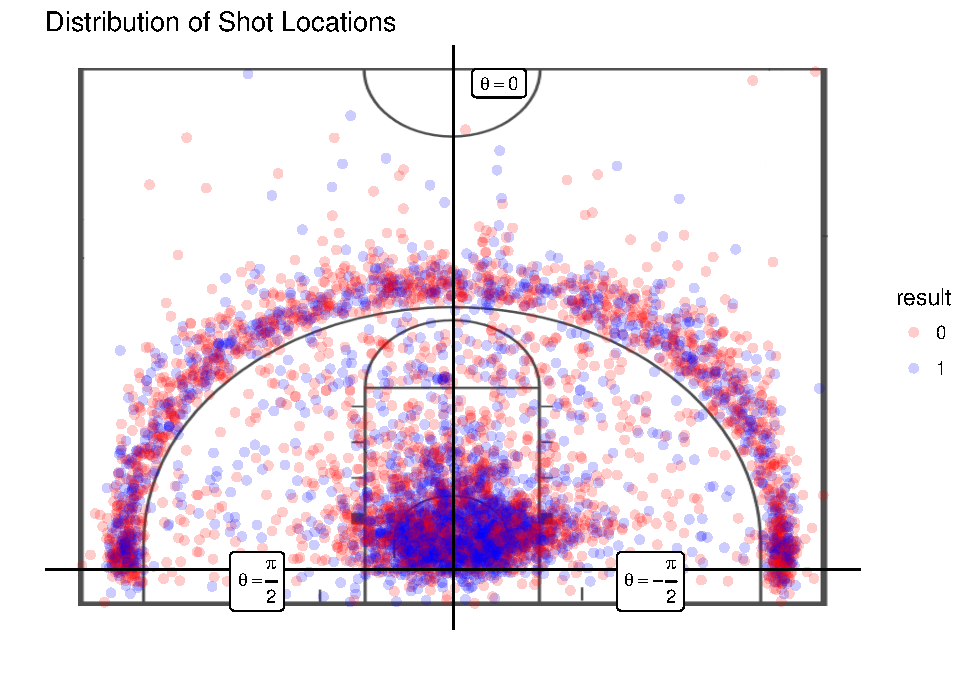
\includegraphics{03-data_files/figure-latex/shotplot-1.pdf}
\caption{\label{fig:shotplot}Locations and Results of All Shots}
\end{figure}
\section{Exploratory Data Analysis}\label{exploratory-data-analysis}

The following exploratory plots in Figure \ref{fig:plots} examine how
consistent the probability of a made shot is, using a loess smooth curve
on the binary outcomes. We present these smoothed plots for four
high-usage basketball players at Duke University between the 2013-2014
and 2016-2017 seasons, and we leave the others in Appendix
\textbf{number}. Each plot represents a single player's ordered shooting
outcomes for a single season. These plots do not account for the amount
of time in between shots, but simply shot order and outcome.
\begin{figure}[htbp]
\centering
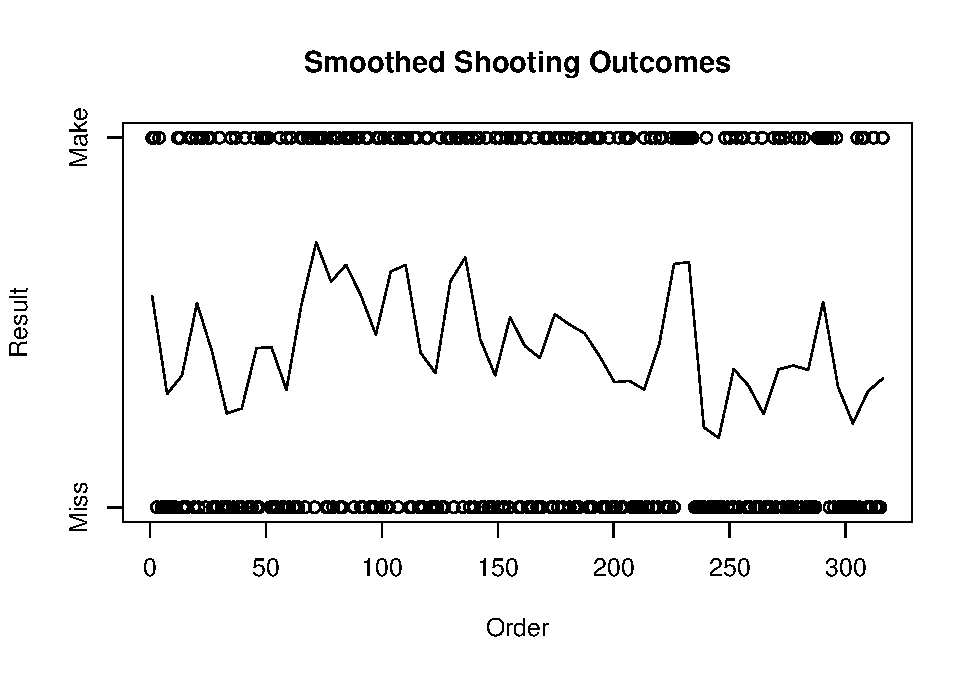
\includegraphics{03-data_files/figure-latex/plots-1.pdf}
\caption{\label{fig:plots}Moving Average of Shot Success Rate}
\end{figure}
We can see that the plots vary in the consistency of their made shots,
since they all contain spikes and trends. For example, the third plot
initially has a very high success rate, which quickly falls to the
middle after about thirty shot attempts, and the second plot has a
noticeable upward trend in shot success beginning around shot number one
hundred fifty.

We investigate the shooting outcomes using Bayesian models, and present
the results in the next section.


% Index?

\end{document}
